\documentclass{article}

\usepackage{Zelig}



\usepackage{Sweave}
\begin{document}
\nobibliography*

\section{{\tt normal}: Normal Regression for Continuous Dependent Variables}
\label{normal}

The Normal regression model is a close variant of the more standard
least squares regression model (see \Sref{ls}). Both models specify a
continuous dependent variable as a linear function of a set of
explanatory variables.  The Normal model reports maximum likelihood
(rather than least squares) estimates.  The two models differ only in
their estimate for the stochastic parameter $\sigma$.

\subsubsection{Syntax}

\begin{verbatim}
> z.out <- zelig(Y ~ X1 + X2, model = "normal", data = mydata)
> x.out <- setx(z.out)
> s.out <- sim(z.out, x = x.out)
\end{verbatim}

\subsubsection{Additional Inputs} 

In addition to the standard inputs, {\tt zelig()} takes the following
additional options for normal regression:  
\begin{itemize}
\item {\tt robust}: defaults to {\tt FALSE}.  If {\tt TRUE} is
selected, {\tt zelig()} computes robust standard errors via the {\tt
sandwich} package (see \cite{Zeileis04}).  The default type of robust
standard error is heteroskedastic and autocorrelation consistent (HAC),
and assumes that observations are ordered by time index.

In addition, {\tt robust} may be a list with the following options:  
\begin{itemize}
\item {\tt method}:  Choose from 
\begin{itemize}
\item {\tt "vcovHAC"}: (default if {\tt robust = TRUE}) HAC standard
errors. 
\item {\tt "kernHAC"}: HAC standard errors using the
weights given in \cite{Andrews91}. 
\item {\tt "weave"}: HAC standard errors using the
weights given in \cite{LumHea99}.  
\end{itemize}  
\item {\tt order.by}: defaults to {\tt NULL} (the observations are
chronologically ordered as in the original data).  Optionally, you may
specify a vector of weights (either as {\tt order.by = z}, where {\tt
z} exists outside the data frame; or as {\tt order.by = \~{}z}, where
{\tt z} is a variable in the data frame).  The observations are
chronologically ordered by the size of {\tt z}.
\item {\tt \dots}:  additional options passed to the functions 
specified in {\tt method}.   See the {\tt sandwich} library and
\cite{Zeileis04} for more options.   
\end{itemize}
\end{itemize}

\subsubsection{Examples}

\begin{enumerate}
\item Basic Example with First Differences

Attach sample data: 
\begin{Schunk}
\begin{Sinput}
> data(macro)
\end{Sinput}
\end{Schunk}
Estimate model:  
\begin{Schunk}
\begin{Sinput}
> z.out1 <- zelig(unem ~ gdp + capmob + trade, model = "normal", 
+     data = macro)
\end{Sinput}
\end{Schunk}
Summarize of regression coefficients:  
\begin{Schunk}
\begin{Sinput}
> summary(z.out1)
\end{Sinput}
\end{Schunk}
Set explanatory variables to their default (mean/mode) values, with
high (80th percentile) and low (20th percentile) values for trade: 
\begin{Schunk}
\begin{Sinput}
> x.high <- setx(z.out1, trade = quantile(macro$trade, 0.8))
> x.low <- setx(z.out1, trade = quantile(macro$trade, 0.2))
\end{Sinput}
\end{Schunk}
Generate first differences for the effect of high versus low trade on
GDP: 
\begin{Schunk}
\begin{Sinput}
> s.out1 <- sim(z.out1, x = x.high, x1 = x.low)
\end{Sinput}
\end{Schunk}
\begin{Schunk}
\begin{Sinput}
> summary(s.out1)
\end{Sinput}
\end{Schunk}
%plot does not work 
A visual summary of quantities of interest:  
\begin{center}
\begin{Schunk}
\begin{Sinput}
> plot(s.out1)
\end{Sinput}
\end{Schunk}
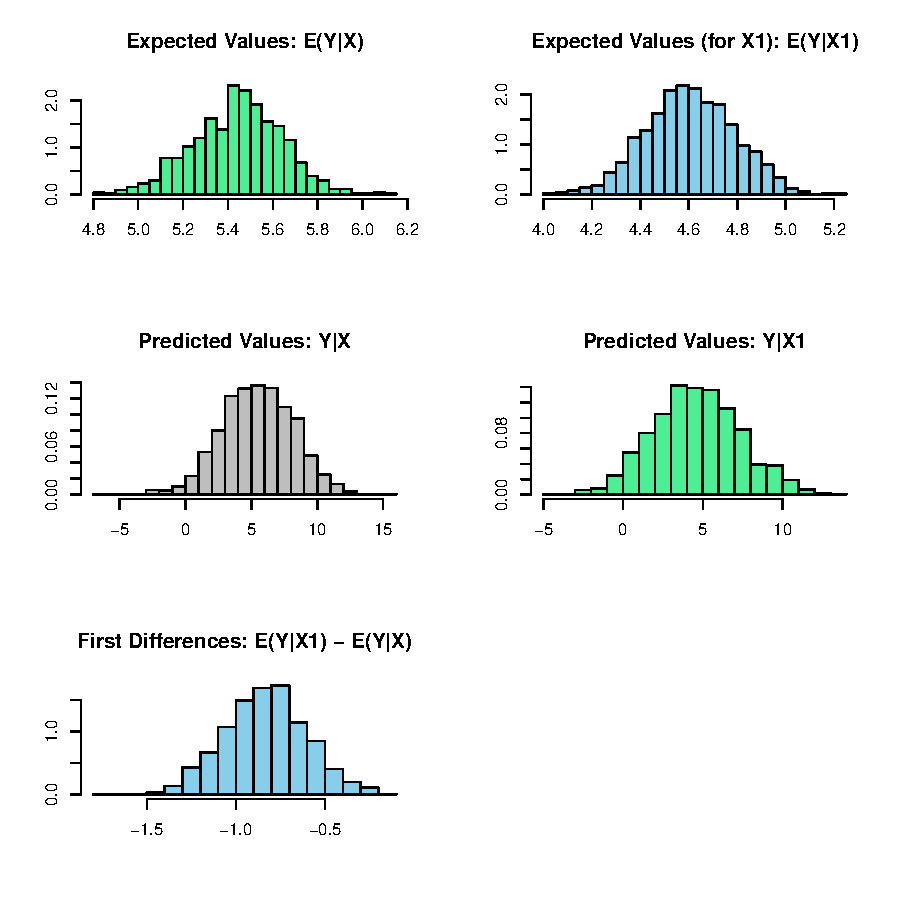
\includegraphics{vigpics/normal-ExamplesPlot}
\end{center}

\item Using Dummy Variables
%the code in this section does not work well but there is no demo for this part either
 
Estimate a model with a dummy variable for each year and country (see
\ref{factors} for help with dummy variables).  Note that you do not
need to create dummy variables, as the program will automatically
parse the unique values in the selected variables into dummy
variables.    
\begin{Schunk}
\begin{Sinput}
> z.out2 <- zelig(unem ~ gdp + trade + capmob + as.factor(year) + 
+     as.factor(country), model = "normal", data = macro)
\end{Sinput}
\end{Schunk}
Set values for the explanatory variables, using the default mean/mode
variables, with country set to the United States and Japan,
respectively: 
Simulate quantities of interest:  
%plot does not work 
\begin{center}
\end{center}
\end{enumerate}

\subsubsection{Model}
Let $Y_i$ be the continuous dependent variable for observation $i$.
\begin{itemize}
\item The \emph{stochastic component} is described by a univariate normal
  model with a vector of means $\mu_i$ and scalar variance $\sigma^2$:
  \begin{equation*}
    Y_i \; \sim \; \textrm{Normal}(\mu_i, \sigma^2). 
  \end{equation*}

\item The \emph{systematic component} is 
  \begin{equation*}
    \mu_i \;= \; x_i \beta,
  \end{equation*}
  where $x_i$ is the vector of $k$ explanatory variables and $\beta$ is
  the vector of coefficients.
\end{itemize}


\subsubsection{Quantities of Interest}

\begin{itemize}
\item The expected value ({\tt qi\$ev}) is the mean of simulations
  from the the stochastic component, $$E(Y) = \mu_i = x_i \beta,$$
  given a draw of $\beta$ from its posterior.  

\item The predicted value ({\tt qi\$pr}) is drawn from the distribution
  defined by the set of parameters $(\mu_i, \sigma)$.  

\item The first difference ({\tt qi\$fd}) is:
\begin{equation*}
\textrm{FD}\; = \;E(Y \mid x_1) -  E(Y \mid x)
\end{equation*}

\item In conditional prediction models, the average expected treatment
  effect ({\tt att.ev}) for the treatment group is 
    \begin{equation*} \frac{1}{\sum_{i=1}^n t_i}\sum_{i:t_i=1}^n \left\{ Y_i(t_i=1) -
      E[Y_i(t_i=0)] \right\},
    \end{equation*} 
    where $t_i$ is a binary explanatory variable defining the treatment
    ($t_i=1$) and control ($t_i=0$) groups.  Variation in the
    simulations are due to uncertainty in simulating $E[Y_i(t_i=0)]$,
    the counterfactual expected value of $Y_i$ for observations in the
    treatment group, under the assumption that everything stays the
    same except that the treatment indicator is switched to $t_i=0$.

\item In conditional prediction models, the average predicted treatment
  effect ({\tt att.pr}) for the treatment group is 
    \begin{equation*} \frac{1}{\sum_{i=1}^n t_i}\sum_{i:t_i=1}^n \left\{ Y_i(t_i=1) -
      \widehat{Y_i(t_i=0)} \right\},
    \end{equation*} 
    where $t_i$ is a binary explanatory variable defining the
    treatment ($t_i=1$) and control ($t_i=0$) groups.  Variation in
    the simulations are due to uncertainty in simulating
    $\widehat{Y_i(t_i=0)}$, the counterfactual predicted value of
    $Y_i$ for observations in the treatment group, under the
    assumption that everything stays the same except that the
    treatment indicator is switched to $t_i=0$.

\end{itemize}

\subsubsection{Output Values}

The output of each Zelig command contains useful information which you
may view.  For example, if you run \texttt{z.out <- zelig(y \~\,
  x, model = "normal", data)}, then you may examine the available
information in \texttt{z.out} by using \texttt{names(z.out)},
see the {\tt coefficients} by using {\tt z.out\$coefficients}, and
a default summary of information through \texttt{summary(z.out)}.
Other elements available through the {\tt \$} operator are listed
below.

\begin{itemize}
\item From the {\tt zelig()} output object {\tt z.out}, you may extract:
   \begin{itemize}
   \item {\tt coefficients}: parameter estimates for the explanatory
     variables.
   \item {\tt residuals}: the working residuals in the final iteration
     of the IWLS fit.
   \item {\tt fitted.values}: fitted values.  For the normal model,
     these are identical to the {\tt linear predictors}.
   \item {\tt linear.predictors}: fitted values.  For the normal
     model, these are identical to {\tt fitted.values}.
   \item {\tt aic}: Akaike's Information Criterion (minus twice the
     maximized log-likelihood plus twice the number of coefficients).
   \item {\tt df.residual}: the residual degrees of freedom.
   \item {\tt df.null}: the residual degrees of freedom for the null
     model.
   \item {\tt zelig.data}: the input data frame if {\tt save.data = TRUE}.  
   \end{itemize}

\item From {\tt summary(z.out)}, you may extract: 
   \begin{itemize}
   \item {\tt coefficients}: the parameter estimates with their
     associated standard errors, $p$-values, and $t$-statistics.
   \item{\tt cov.scaled}: a $k \times k$ matrix of scaled covariances.
   \item{\tt cov.unscaled}: a $k \times k$ matrix of unscaled
     covariances.  
   \end{itemize}

\item From the {\tt sim()} output object {\tt s.out}, you may extract
  quantities of interest arranged as matrices indexed by simulation
  $\times$ {\tt x}-observation (for more than one {\tt x}-observation).
  Available quantities are:

   \begin{itemize}
   \item {\tt qi\$ev}: the simulated expected values for the specified
     values of {\tt x}.
   \item {\tt qi\$pr}: the simulated predicted values drawn from the
     distribution defined by $(\mu_i, \sigma)$.
   \item {\tt qi\$fd}: the simulated first difference in the simulated
     expected values for the values specified in {\tt x} and {\tt x1}.
   \item {\tt qi\$att.ev}: the simulated average expected treatment
     effect for the treated from conditional prediction models.  
   \item {\tt qi\$att.pr}: the simulated average predicted treatment
     effect for the treated from conditional prediction models.  
   \end{itemize}
\end{itemize}

\subsection* {How to Cite} 

How to cite this model in Zelig:
\begin{verse}
  Kosuke Imai, Gary King, and Olivia Lau. 2008. "normal: Normal Regression for Continuous Dependent Variables" in Kosuke Imai, Gary King, and Olivia Lau, "Zelig: Everyone's Statistical Software,"http://gking.harvard.edu/zelig
\end{verse}

\CiteZelig

\subsection* {See also}

The normal model is part of the stats package by \citet{VenRip02}.
Advanced users may wish to refer to \texttt{help(glm)} and
\texttt{help(family)}, as well as \cite{McCNel89}. Robust standard
errors are implemented via the sandwich package by \citet{Zeileis04}.
Sample data are from \cite{KinTomWit00}.

\bibliographystyle{asa}
\bibliography{gk,gkpubs}
 \end{document}


%%% Local Variables: 
%%% mode: latex
%%% TeX-master: t
%%% End: 












